\documentclass[../Main.tex]{subfiles}

\begin{document}
\author{Voltage and Resistance} %use author for title of lesson
\date{Year 1 Topic 11} %use date to refer to topic in main booklet

\section{Voltage and Resistance} %Section is the title of the lesson repeated, ready for the main contents page.

\begin{frame}{Current}
    Previously we have said current is a charge moving. With regards to electricity in general these are electrons flowing through a wire (remember that it can be \emph{any} charged particle!)
    \newline
    
    But what actually makes the electrons move? If initially electrons are `stationary in a battery' (THIS IS NOT TRUE), what is the driving force that pushes them round a circuit?
\end{frame}

\begin{frame}{Voltage}
    We say there is an electromotive force (emf) -- note that it is not technically a force -- pushing electrons around a circuit (you do not need to mention this in any exam question).
    
    \begin{block}{Voltage}
Also known as potential difference or sometimes just referred to as the emf, voltage is a measure of the work done in creating a current. It is the work done per unit charge. You could think of this as an attempt to push electrons round a circuit.
    \end{block}
    
    \begin{equation*}
        V = \frac{W}{Q}
    \end{equation*}
     1 Volt is defined as 1 Joule of work being carried out on 1 Coulomb of charge.
    \begin{exampleblock}{Exam Tip}
    If you get asked to define the volt, use the above formula to help remember!
    \end{exampleblock}
\end{frame}

\begin{frame}{Examples}

\begin{equation*}
    V=\frac{W}{Q}
\end{equation*}
    \begin{exampleblock}{Example}
    An phone charger uses 2400 J of energy and delivers 12 V of potential difference. Calculate the charge transferred to the phone battery. \newline \pause
    --200C
    \end{exampleblock}
    
    \pause 
    Your turn! Try out some Kerboodle Questions (from page 138)
    \begin{figure}
        \centering
        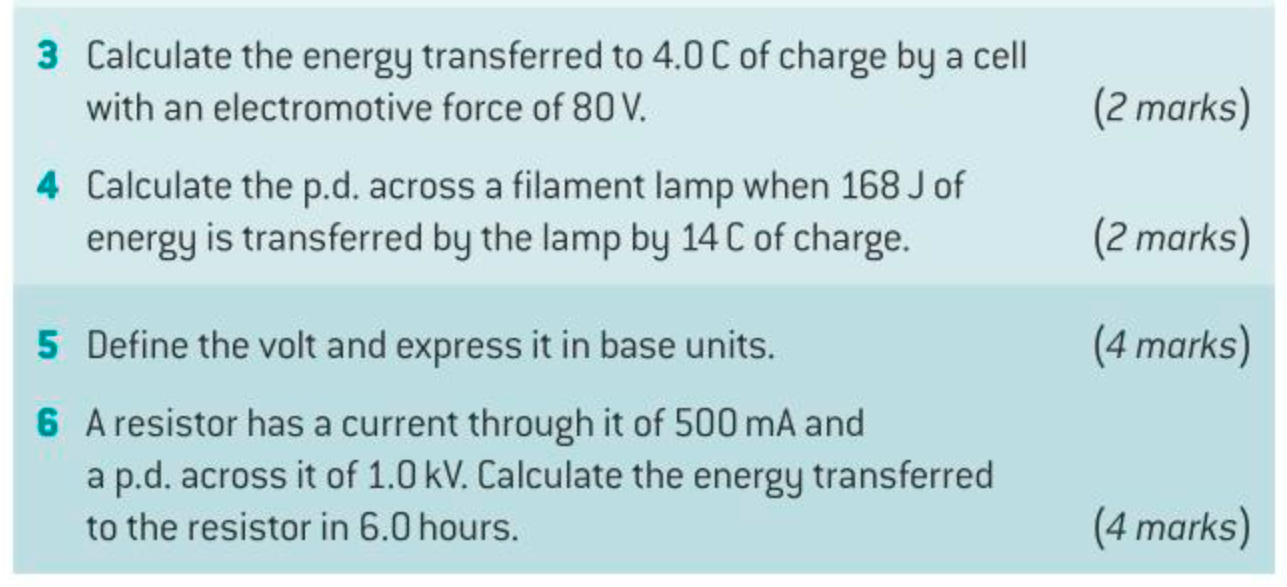
\includegraphics[height=3cm]{Electricity_Images/kerboodle_Qs_voltage.png}
    \end{figure}
\end{frame}

\begin{frame}{Resistance}
    \begin{block}{Resistance}
    Resistance is a measure of how easy/hard it is to make a current flow. It has units \emph{Ohms} ($\Omega$).
    \end{block}
    \begin{multicols}{2}
    \begin{equation*}
        V=IR
    \end{equation*}
    
     Increasing the resistance will decrease the current -- to combat this you need more voltage, i.e. you need to do more work on the electrons. This is \emph{Ohm's law}.
\columnbreak
     \begin{figure}
         \centering
         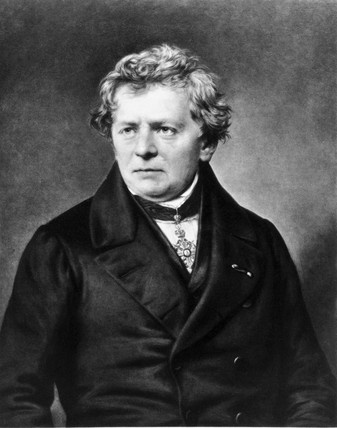
\includegraphics[width=3.5cm]{Electricity_Images/Georg_Simon_Ohm.jpg}
         \caption{Georg Ohm}
     \end{figure}
     \end{multicols}
\end{frame}

\begin{frame}{Ohm's Law}
    More formally, 
    
    \begin{block}{Ohm's Law}
    Ohm's law states that the current in a circuit is directly proportional to the voltage supplied, and inversely proportional to the total resistance in the circuit.
    \end{block}
    \begin{figure}
        \centering
        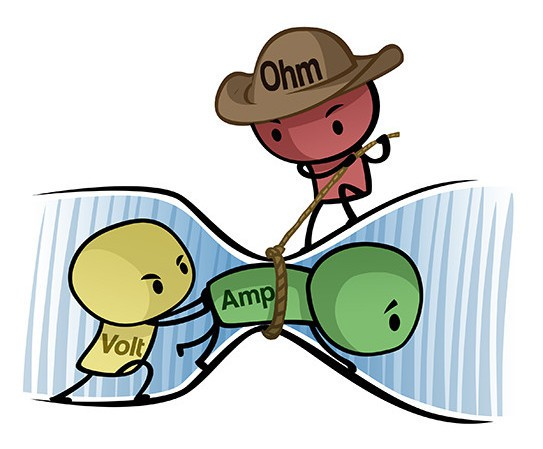
\includegraphics[height=4.5cm]{Electricity_Images/ohms_law.jpg}
    \end{figure}
\end{frame}

\begin{frame}{Example}
\newline {\large
\begin{equation*}
    V=IR
\end{equation*}}
    \begin{exampleblock}{Example}
    An electric kettle uses mains voltage (230V). The current is 10A. What is the resistance? \pause
    --23$\Omega$
    \end{exampleblock}
    Big one to remember -- mains voltage is 230V!
    \pause
    \begin{exampleblock}{Challenge}
    Determine the SI unit for resistance - you may need to look back at some other equations to help you! \pause 
    --$kgm^2A^{-2}s^{-3}$ {\tiny(you do not need to know this, though)}
    \end{exampleblock}
    \pause
    Now try some on Kerboodle page 143
\end{frame}

\end{document}